% Created by tikzDevice version 0.11 on 2018-04-15 12:26:50
% !TEX encoding = UTF-8 Unicode
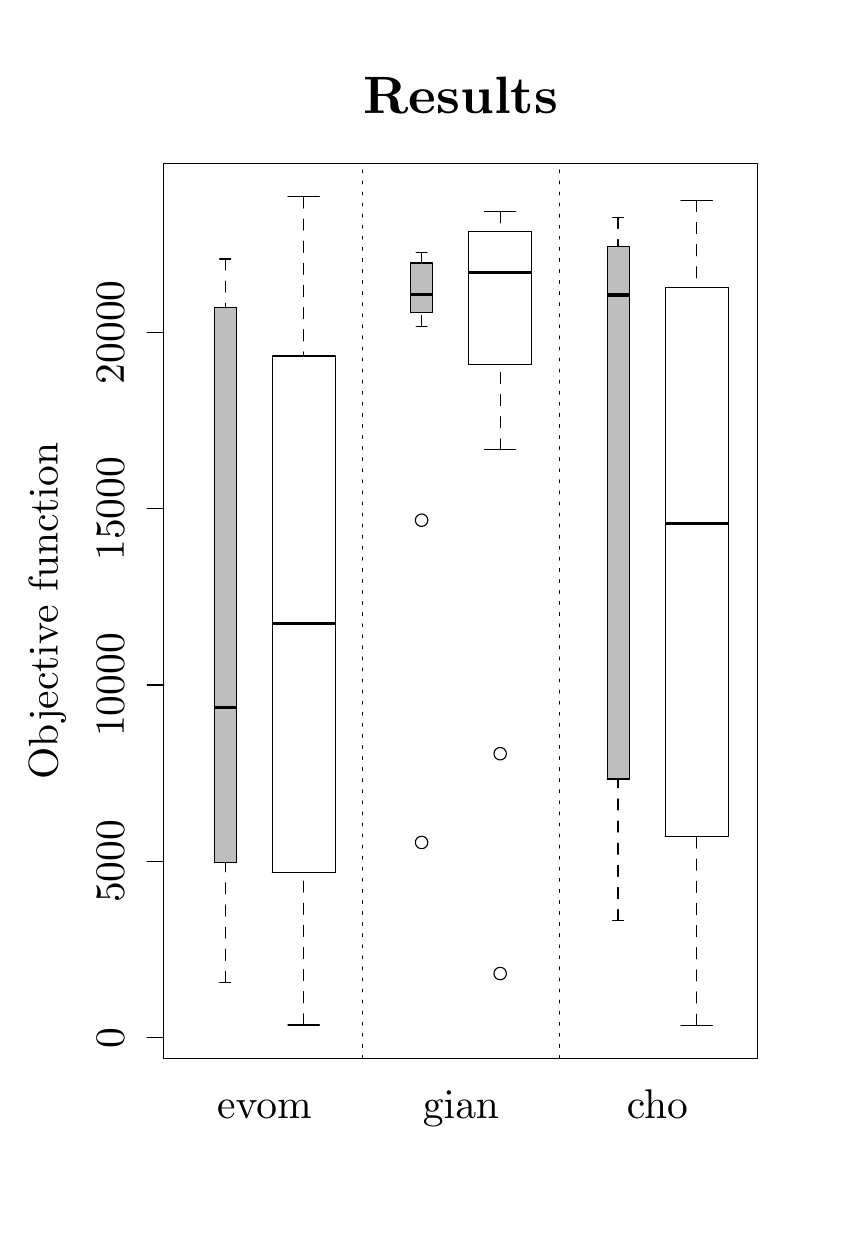
\begin{tikzpicture}[x=1pt,y=1pt]
\definecolor{fillColor}{RGB}{255,255,255}
\path[use as bounding box,fill=fillColor,fill opacity=0.00] (0,0) rectangle (289.08,433.62);
\begin{scope}
\path[clip] ( 49.20, 61.20) rectangle (263.88,384.42);
\definecolor{fillColor}{RGB}{190,190,190}

\path[fill=fillColor] ( 67.37,131.97) --
	( 75.33,131.97) --
	( 75.33,332.40) --
	( 67.37,332.40) --
	cycle;
\definecolor{drawColor}{RGB}{0,0,0}

\path[draw=drawColor,line width= 1.2pt,line join=round] ( 67.37,188.08) -- ( 75.33,188.08);

\path[draw=drawColor,line width= 0.4pt,dash pattern=on 4pt off 4pt ,line join=round,line cap=round] ( 71.35, 88.62) -- ( 71.35,131.97);

\path[draw=drawColor,line width= 0.4pt,dash pattern=on 4pt off 4pt ,line join=round,line cap=round] ( 71.35,350.04) -- ( 71.35,332.40);

\path[draw=drawColor,line width= 0.4pt,line join=round,line cap=round] ( 69.36, 88.62) -- ( 73.34, 88.62);

\path[draw=drawColor,line width= 0.4pt,line join=round,line cap=round] ( 69.36,350.04) -- ( 73.34,350.04);

\path[draw=drawColor,line width= 0.4pt,line join=round,line cap=round] ( 67.37,131.97) --
	( 75.33,131.97) --
	( 75.33,332.40) --
	( 67.37,332.40) --
	( 67.37,131.97);
\definecolor{fillColor}{RGB}{255,255,255}

\path[fill=fillColor] ( 88.39,128.34) --
	(111.11,128.34) --
	(111.11,314.97) --
	( 88.39,314.97) --
	cycle;

\path[draw=drawColor,line width= 1.2pt,line join=round] ( 88.39,218.37) -- (111.11,218.37);

\path[draw=drawColor,line width= 0.4pt,dash pattern=on 4pt off 4pt ,line join=round,line cap=round] ( 99.75, 73.25) -- ( 99.75,128.34);

\path[draw=drawColor,line width= 0.4pt,dash pattern=on 4pt off 4pt ,line join=round,line cap=round] ( 99.75,372.45) -- ( 99.75,314.97);

\path[draw=drawColor,line width= 0.4pt,line join=round,line cap=round] ( 94.07, 73.25) -- (105.43, 73.25);

\path[draw=drawColor,line width= 0.4pt,line join=round,line cap=round] ( 94.07,372.45) -- (105.43,372.45);

\path[draw=drawColor,line width= 0.4pt,line join=round,line cap=round] ( 88.39,128.34) --
	(111.11,128.34) --
	(111.11,314.97) --
	( 88.39,314.97) --
	( 88.39,128.34);
\definecolor{fillColor}{RGB}{190,190,190}

\path[fill=fillColor] (138.37,330.70) --
	(146.32,330.70) --
	(146.32,348.57) --
	(138.37,348.57) --
	cycle;

\path[draw=drawColor,line width= 1.2pt,line join=round] (138.37,337.09) -- (146.32,337.09);

\path[draw=drawColor,line width= 0.4pt,dash pattern=on 4pt off 4pt ,line join=round,line cap=round] (142.34,325.66) -- (142.34,330.70);

\path[draw=drawColor,line width= 0.4pt,dash pattern=on 4pt off 4pt ,line join=round,line cap=round] (142.34,352.37) -- (142.34,348.57);

\path[draw=drawColor,line width= 0.4pt,line join=round,line cap=round] (140.35,325.66) -- (144.33,325.66);

\path[draw=drawColor,line width= 0.4pt,line join=round,line cap=round] (140.35,352.37) -- (144.33,352.37);

\path[draw=drawColor,line width= 0.4pt,line join=round,line cap=round] (138.37,330.70) --
	(146.32,330.70) --
	(146.32,348.57) --
	(138.37,348.57) --
	(138.37,330.70);

\path[draw=drawColor,line width= 0.4pt,line join=round,line cap=round] (142.34,255.64) circle (  2.25);

\path[draw=drawColor,line width= 0.4pt,line join=round,line cap=round] (142.34,139.19) circle (  2.25);
\definecolor{fillColor}{RGB}{255,255,255}

\path[fill=fillColor] (159.38,311.84) --
	(182.10,311.84) --
	(182.10,359.95) --
	(159.38,359.95) --
	cycle;

\path[draw=drawColor,line width= 1.2pt,line join=round] (159.38,345.15) -- (182.10,345.15);

\path[draw=drawColor,line width= 0.4pt,dash pattern=on 4pt off 4pt ,line join=round,line cap=round] (170.74,281.03) -- (170.74,311.84);

\path[draw=drawColor,line width= 0.4pt,dash pattern=on 4pt off 4pt ,line join=round,line cap=round] (170.74,367.12) -- (170.74,359.95);

\path[draw=drawColor,line width= 0.4pt,line join=round,line cap=round] (165.06,281.03) -- (176.42,281.03);

\path[draw=drawColor,line width= 0.4pt,line join=round,line cap=round] (165.06,367.12) -- (176.42,367.12);

\path[draw=drawColor,line width= 0.4pt,line join=round,line cap=round] (159.38,311.84) --
	(182.10,311.84) --
	(182.10,359.95) --
	(159.38,359.95) --
	(159.38,311.84);

\path[draw=drawColor,line width= 0.4pt,line join=round,line cap=round] (170.74, 91.83) circle (  2.25);

\path[draw=drawColor,line width= 0.4pt,line join=round,line cap=round] (170.74,171.27) circle (  2.25);
\definecolor{fillColor}{RGB}{190,190,190}

\path[fill=fillColor] (209.36,162.13) --
	(217.31,162.13) --
	(217.31,354.67) --
	(209.36,354.67) --
	cycle;

\path[draw=drawColor,line width= 1.2pt,line join=round] (209.36,337.07) -- (217.31,337.07);

\path[draw=drawColor,line width= 0.4pt,dash pattern=on 4pt off 4pt ,line join=round,line cap=round] (213.33,110.94) -- (213.33,162.13);

\path[draw=drawColor,line width= 0.4pt,dash pattern=on 4pt off 4pt ,line join=round,line cap=round] (213.33,365.06) -- (213.33,354.67);

\path[draw=drawColor,line width= 0.4pt,line join=round,line cap=round] (211.35,110.94) -- (215.32,110.94);

\path[draw=drawColor,line width= 0.4pt,line join=round,line cap=round] (211.35,365.06) -- (215.32,365.06);

\path[draw=drawColor,line width= 0.4pt,line join=round,line cap=round] (209.36,162.13) --
	(217.31,162.13) --
	(217.31,354.67) --
	(209.36,354.67) --
	(209.36,162.13);
\definecolor{fillColor}{RGB}{255,255,255}

\path[fill=fillColor] (230.37,141.40) --
	(253.09,141.40) --
	(253.09,339.57) --
	(230.37,339.57) --
	cycle;

\path[draw=drawColor,line width= 1.2pt,line join=round] (230.37,254.54) -- (253.09,254.54);

\path[draw=drawColor,line width= 0.4pt,dash pattern=on 4pt off 4pt ,line join=round,line cap=round] (241.73, 73.17) -- (241.73,141.40);

\path[draw=drawColor,line width= 0.4pt,dash pattern=on 4pt off 4pt ,line join=round,line cap=round] (241.73,371.21) -- (241.73,339.57);

\path[draw=drawColor,line width= 0.4pt,line join=round,line cap=round] (236.05, 73.17) -- (247.41, 73.17);

\path[draw=drawColor,line width= 0.4pt,line join=round,line cap=round] (236.05,371.21) -- (247.41,371.21);

\path[draw=drawColor,line width= 0.4pt,line join=round,line cap=round] (230.37,141.40) --
	(253.09,141.40) --
	(253.09,339.57) --
	(230.37,339.57) --
	(230.37,141.40);
\end{scope}
\begin{scope}
\path[clip] (  0.00,  0.00) rectangle (289.08,433.62);
\definecolor{drawColor}{RGB}{0,0,0}

\node[text=drawColor,rotate= 90.00,anchor=base,inner sep=0pt, outer sep=0pt, scale=  1.50] at ( 10.80,222.81) {Objective function};
\end{scope}
\begin{scope}
\path[clip] ( 49.20, 61.20) rectangle (263.88,384.42);
\definecolor{drawColor}{RGB}{0,0,0}

\path[draw=drawColor,line width= 0.4pt,dash pattern=on 1pt off 3pt ,line join=round,line cap=round] (121.04, 61.20) -- (121.04,384.42);

\path[draw=drawColor,line width= 0.4pt,dash pattern=on 1pt off 3pt ,line join=round,line cap=round] (192.04, 61.20) -- (192.04,384.42);
\end{scope}
\begin{scope}
\path[clip] (  0.00,  0.00) rectangle (289.08,433.62);
\definecolor{drawColor}{RGB}{0,0,0}

\node[text=drawColor,anchor=base,inner sep=0pt, outer sep=0pt, scale=  1.50] at ( 85.55, 39.60) {evom};

\node[text=drawColor,anchor=base,inner sep=0pt, outer sep=0pt, scale=  1.50] at (156.54, 39.60) {gian};

\node[text=drawColor,anchor=base,inner sep=0pt, outer sep=0pt, scale=  1.50] at (227.53, 39.60) {cho};
\end{scope}
\begin{scope}
\path[clip] (  0.00,  0.00) rectangle (289.08,433.62);
\definecolor{drawColor}{RGB}{0,0,0}

\node[text=drawColor,anchor=base,inner sep=0pt, outer sep=0pt, scale=  1.90] at (156.54,402.46) {\bfseries Results};
\end{scope}
\begin{scope}
\path[clip] (  0.00,  0.00) rectangle (289.08,433.62);
\definecolor{drawColor}{RGB}{0,0,0}

\path[draw=drawColor,line width= 0.4pt,line join=round,line cap=round] ( 49.20, 68.62) -- ( 49.20,323.53);

\path[draw=drawColor,line width= 0.4pt,line join=round,line cap=round] ( 49.20, 68.62) -- ( 43.20, 68.62);

\path[draw=drawColor,line width= 0.4pt,line join=round,line cap=round] ( 49.20,132.35) -- ( 43.20,132.35);

\path[draw=drawColor,line width= 0.4pt,line join=round,line cap=round] ( 49.20,196.08) -- ( 43.20,196.08);

\path[draw=drawColor,line width= 0.4pt,line join=round,line cap=round] ( 49.20,259.80) -- ( 43.20,259.80);

\path[draw=drawColor,line width= 0.4pt,line join=round,line cap=round] ( 49.20,323.53) -- ( 43.20,323.53);

\node[text=drawColor,rotate= 90.00,anchor=base,inner sep=0pt, outer sep=0pt, scale=  1.50] at ( 34.80, 68.62) {0};

\node[text=drawColor,rotate= 90.00,anchor=base,inner sep=0pt, outer sep=0pt, scale=  1.50] at ( 34.80,132.35) {5000};

\node[text=drawColor,rotate= 90.00,anchor=base,inner sep=0pt, outer sep=0pt, scale=  1.50] at ( 34.80,196.08) {10000};

\node[text=drawColor,rotate= 90.00,anchor=base,inner sep=0pt, outer sep=0pt, scale=  1.50] at ( 34.80,259.80) {15000};

\node[text=drawColor,rotate= 90.00,anchor=base,inner sep=0pt, outer sep=0pt, scale=  1.50] at ( 34.80,323.53) {20000};

\path[draw=drawColor,line width= 0.4pt,line join=round,line cap=round] ( 49.20, 61.20) --
	(263.88, 61.20) --
	(263.88,384.42) --
	( 49.20,384.42) --
	( 49.20, 61.20);
\end{scope}
\end{tikzpicture}
